\documentclass[11pt]{article}
\usepackage[margin=0.75in]{geometry}
\usepackage{graphicx}
\usepackage{booktabs}
\usepackage{float}
\usepackage{hyperref}
\usepackage{amsmath}
\usepackage{longtable}
\usepackage{array}

\title{Computational Prediction of Drug-Induced Heart Damage:\\
ADMET-AI vs SwissADME Comparison\\
\large Analysis of 25 Cardiac RODEO Drugs}
\author{Cardiac RODEO Project}
\date{\today}

\begin{document}
\maketitle

\begin{abstract}
This report compares two computational approaches for predicting drug-induced heart damage:
ADMET-AI (41 ADMET properties) and SwissADME (43 physicochemical properties).
We replicate published DICTrank benchmark results, evaluate predictions on 25 Cardiac RODEO drugs,
and train new models using Leave-One-Out Cross-Validation (LOOCV) and scaffold-balanced CV.
\end{abstract}

\section{DICTrank Model: Training and 25-Drug Inference}

\textbf{Part 1: DICTrank model replication.}
We retrain the published DICTrank models on the DICTrank dataset (555 drugs: 293 most DICT concern, 262 no concern)
using 10-fold scaffold-balanced cross-validation to confirm benchmark performance.

\textbf{Part 2: 25-drug inference.}
We then generate features from the 25 Cardiac RODEO SMILES and pass them through the trained DICTrank models
to obtain DICT concern probabilities (no retraining on the 25-drug set).

\subsection{Process Summary}
\begin{itemize}
    \item \textbf{Training data:} DICTrank 555-drug dataset (most vs no concern).
    \item \textbf{Models:} GradientBoostingClassifier (n\_estimators=500, max\_depth=12, learning\_rate=0.1, random\_state=0).
    \item \textbf{Validation:} 10-fold scaffold-balanced CV; fold test predictions concatenated for ROC/AUC and confusion matrices.
    \item \textbf{Decision rule:} probability $\ge$ 0.5 for DICT concern.
    \item \textbf{25-drug inference:} ADMET-AI features computed for 25 drugs; SwissADME features available for 23 drugs, then passed through the trained DICTrank models (no retraining).
    \item \textbf{SwissADME coverage:*} Dactinomycin and Plicamycin are excluded due to size; SwissADME columns are shown as ``--''.
\end{itemize}

\begin{table}[H]
\centering
\caption{DICTrank Training Results (10-Fold CV)}
\begin{tabular}{lccc}
\toprule
\textbf{Model} & \textbf{ROC AUC} & \textbf{PR AUC} & \textbf{Accuracy} \\
\midrule
ADMET-AI & 0.72 & 0.75 & 0.64 \\
SwissADME & 0.66 & 0.68 & 0.60 \\
\bottomrule
\end{tabular}
\end{table}

\begin{figure}[H]
\centering
\begin{minipage}{0.48\textwidth}
\centering

\includegraphics[width=\textwidth]{figures/dictrank_retrain_roc.pdf}
\end{minipage}
\hfill
\begin{minipage}{0.40\textwidth}
\centering
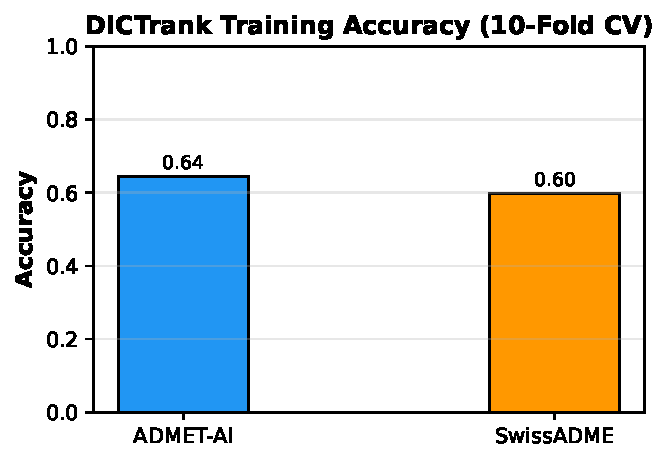
\includegraphics[width=\textwidth]{figures/dictrank_training_accuracy.pdf}
\end{minipage}
\caption{DICTrank training ROC and accuracy (10-fold CV on 555 drugs).}
\end{figure}

\begin{figure}[H]
\centering
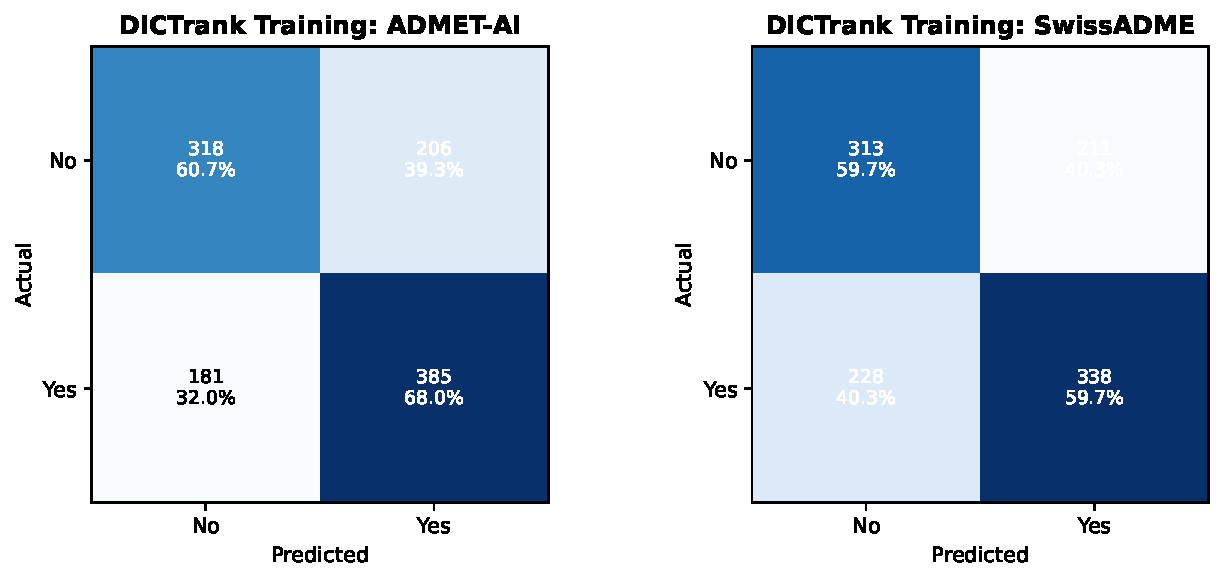
\includegraphics[width=0.85\textwidth]{figures/dictrank_training_confusion.pdf}
\caption{DICTrank training confusion matrices (10-fold CV on 555 drugs).}
\end{figure}


\subsection{Cardiac RODEO Drug Dataset}

Our dataset contains 25 drugs with experimentally determined cardiac outcomes:
\begin{itemize}
    \item Heart Damage Positive: 20/25 drugs (80\\%)
    \item Heart Damage Negative: 5/25 drugs (20\\%)
\end{itemize}

\begin{longtable}{lcc>{\raggedright\arraybackslash}p{7cm}}
\caption{Drug Database with SMILES and Sources} \\
\toprule
\textbf{Drug} & \textbf{CID} & \textbf{MW} & \textbf{SMILES} \\
\midrule
\endfirsthead
\toprule
\textbf{Drug} & \textbf{CID} & \textbf{MW} & \textbf{SMILES} \\
\midrule
\endhead
    Amiodarone & 2157 & 645.3 & \begin{tabular}[t]{@{}l@{}}\texttt{CCCCc1oc2c(c1C(=O)c1cc(I)c(c(c1)I)O}\\\texttt{CCN(CC)CC)cccc2}\end{tabular} \\
    Bortezomib & 387447 & 384.2 & \begin{tabular}[t]{@{}l@{}}\texttt{CC(C[C@@H](B(O)O)NC(=O)[C@@H](NC(=O}\\\texttt{)c1cnccn1)Cc1ccccc1)C}\end{tabular} \\
    Chlorpromazine & 2726 & 318.9 & \begin{tabular}[t]{@{}l@{}}\texttt{CN(CCCN1c2ccccc2Sc2c1cc(Cl)cc2)C}\end{tabular} \\
    Cobimetinib & 16222096 & 531.3 & \begin{tabular}[t]{@{}l@{}}\texttt{Ic1ccc(c(c1)F)Nc1c(ccc(c1F)F)C(=O)N}\\\texttt{1CC(C1)(O)[C@@H]1CCCCN1}\end{tabular} \\
    Dactinomycin & 457193 & 1255.4 & \begin{tabular}[t]{@{}l@{}}\texttt{C[C@@H]1[C@@H](C(=O)N[C@@H](C(=O)N2}\\\texttt{CCC[C@H]2C(=O)N(CC(=O)N([C@H](C(=O)}\\\texttt{O1)C(C)C)C)C)C(C)C)NC(=O)C3=C4C(=C(}\\\texttt{C=C3)C)OC5=C(C(=O)C(=C(C5=N4)C(=O)N}\\\texttt{[C@H]6[C@H](OC(=O)[C@@H](N(C(=O)CN(}\\\texttt{C(=O)[C@@H]7CCCN7C(=O)[C@H](NC6=O)C}\\\texttt{(C)C)C)C)C(C)C)C)N)C}\end{tabular} \\
    Daunorubicin & 30323 & 527.5 & \begin{tabular}[t]{@{}l@{}}\texttt{COc1cccc2c1C(=O)c1c(C2=O)c(O)c2c(c1}\\\texttt{O)[C@@H](O[C@H]1C[C@H](N)[C@@H]([C@}\\\texttt{@H](O1)C)O)C[C@](C2)(O)C(=O)C}\end{tabular} \\
    Doxorubicin & 31703 & 543.5 & \begin{tabular}[t]{@{}l@{}}\texttt{OCC(=O)[C@@]1(O)C[C@H](O[C@H]2C[C@H}\\\texttt{](N)[C@@H]([C@@H](O2)C)O)c2c(C1)c(O}\\\texttt{)c1c(c2O)C(=O)c2c(C1=O)cccc2OC}\end{tabular} \\
    Epirubicin & 41867 & 543.5 & \begin{tabular}[t]{@{}l@{}}\texttt{OCC(=O)[C@@]1(O)C[C@H](O[C@H]2C[C@H}\\\texttt{](N)[C@H]([C@@H](O2)C)O)c2c(C1)c(O)}\\\texttt{c1c(c2O)C(=O)c2c(C1=O)cccc2OC}\end{tabular} \\
    Erlotinib & 176870 & 393.4 & \begin{tabular}[t]{@{}l@{}}\texttt{COCCOc1cc2c(ncnc2cc1OCCOC)Nc1cccc(c}\\\texttt{1)C\#C}\end{tabular} \\
    Etomoxir & 9840324 & 326.8 & \begin{tabular}[t]{@{}l@{}}\texttt{CCOC(=O)[C@]1(CCCCCCOc2ccc(cc2)Cl)O}\\\texttt{C1}\end{tabular} \\
    Gemcitibine & 60750 & 263.2 & \begin{tabular}[t]{@{}l@{}}\texttt{OC[C@H]1O[C@H](C([C@@H]1O)(F)F)n1cc}\\\texttt{c(nc1=O)N}\end{tabular} \\
    Ibrutinib & 24821094 & 440.5 & \begin{tabular}[t]{@{}l@{}}\texttt{C=CC(=O)N1CCC[C@H](C1)n1nc(c2c1ncnc}\\\texttt{2N)c1ccc(cc1)Oc1ccccc1}\end{tabular} \\
    Ibuprofen & 3672 & 206.3 & \begin{tabular}[t]{@{}l@{}}\texttt{CC(Cc1ccc(cc1)C(C(=O)O)C)C}\end{tabular} \\
    Isoproterenol & 3779 & 211.3 & \begin{tabular}[t]{@{}l@{}}\texttt{CC(NCC(c1ccc(c(c1)O)O)O)C}\end{tabular} \\
    Mexiletine & 4178 & 179.3 & \begin{tabular}[t]{@{}l@{}}\texttt{CC(COc1c(C)cccc1C)N}\end{tabular} \\
    Nifedipine & 4485 & 346.3 & \begin{tabular}[t]{@{}l@{}}\texttt{COC(=O)C1=C(C)NC(=C(C1c1ccccc1[N+](}\\\texttt{=O)[O-])C(=O)OC)C}\end{tabular} \\
    Panobinostat & 6918837 & 349.4 & \begin{tabular}[t]{@{}l@{}}\texttt{ONC(=O)/C=C/c1ccc(cc1)CNCCc1c(C)[nH}\\\texttt{]c2c1cccc2}\end{tabular} \\
    Plicamycin & 163659 & 1085.1 & \begin{tabular}[t]{@{}l@{}}\texttt{C[C@@H]1[C@H]([C@@H](C[C@@H](O1)O[C}\\\texttt{@@H]2C[C@@H](O[C@@H]([C@H]2O)C)OC3=}\\\texttt{CC4=CC5=C(C(=O)[C@H]([C@@H](C5)[C@@}\\\texttt{H](C(=O)[C@H]([C@@H](C)O)O)OC)O[C@H}\\\texttt{]6C[C@H]([C@@H]([C@H](O6)C)O)O[C@H]}\\\texttt{7C[C@H]([C@H]([C@H](O7)C)O)O[C@H]8C}\\\texttt{[C@]([C@@H]([C@H](O8)C)O)(C)O)C(=C4}\\\texttt{C(=C3C)O)O)O)O}\end{tabular} \\
    Rosiglitazone & 77999 & 357.4 & \begin{tabular}[t]{@{}l@{}}\texttt{O=C1NC(=O)C(S1)Cc1ccc(cc1)OCCN(c1cc}\\\texttt{ccn1)C}\end{tabular} \\
    Sotalol & 5253 & 272.4 & \begin{tabular}[t]{@{}l@{}}\texttt{CC(NCC(c1ccc(cc1)NS(=O)(=O)C)O)C}\end{tabular} \\
    Sunitinib & 5329102 & 398.5 & \begin{tabular}[t]{@{}l@{}}\texttt{CCN(CCNC(=O)c1c(C)[nH]c(c1C)/C=C/1\textbackslash\{\}}\\\texttt{C(=O)Nc2c1cc(F)cc2)CC}\end{tabular} \\
    Vandetanib & 3081361 & 475.4 & \begin{tabular}[t]{@{}l@{}}\texttt{COc1cc2c(ncnc2cc1OCC1CCN(CC1)C)Nc1c}\\\texttt{cc(cc1F)Br}\end{tabular} \\
    Vincristine & 5978 & 825.0 & \begin{tabular}[t]{@{}l@{}}\texttt{O=CN1c2cc(OC)c(cc2[C@]23[C@@H]1[C@@}\\\texttt{](O)(C(=O)OC)[C@H](OC(=O)C)[C@]1([C}\\\texttt{@@H]3N(CC2)CC=C1)CC)[C@]1(C[C@@H]2C}\\\texttt{N(CCc3c1[nH]c1c3cccc1)C[C@](C2)(O)C}\\\texttt{C)C(=O)OC}\end{tabular} \\
    Vioxx & 5090 & 314.4 & \begin{tabular}[t]{@{}l@{}}\texttt{O=C1OCC(=C1c1ccccc1)c1ccc(cc1)S(=O)}\\\texttt{(=O)C}\end{tabular} \\
    Vorinostat & 5311 & 264.3 & \begin{tabular}[t]{@{}l@{}}\texttt{ONC(=O)CCCCCCC(=O)Nc1ccccc1}\end{tabular} \\
\bottomrule
\end{longtable}

All drugs sourced from PubChem (https://pubchem.ncbi.nlm.nih.gov).

\subsection{DICTrank Inference on 25 Drugs}

\begin{table}[H]
\centering
\caption{DICTrank Model Performance (ADMET-AI: 25 drugs, SwissADME: 23 drugs)}
\begin{tabular}{lcccccc}
\toprule
\textbf{Model} & \textbf{Accuracy} & \textbf{ROC AUC} & \textbf{TP} & \textbf{FN} & \textbf{TN} & \textbf{FP} \\
\midrule
ADMET-AI & 0.56 & 0.45 & 12 & 8 & 2 & 3 \\
SwissADME & 0.57 & 0.60 & 11 & 9 & 2 & 1 \\
\bottomrule
\end{tabular}
\end{table}

\begin{figure}[H]
\centering
\begin{minipage}{0.40\textwidth}
\centering
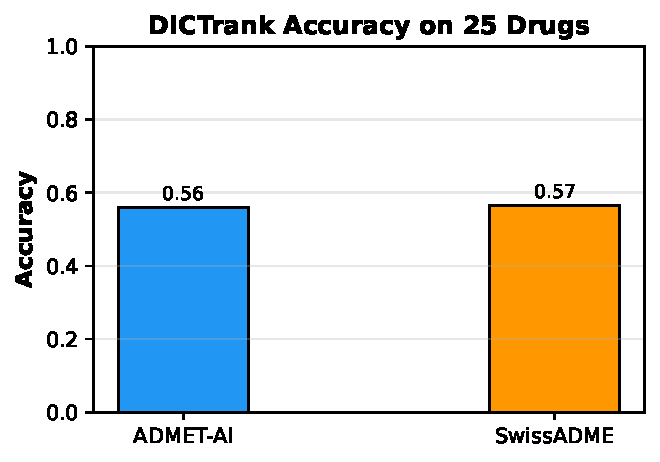
\includegraphics[width=\textwidth]{figures/dictrank_accuracy_bar.pdf}
\end{minipage}
\hfill
\begin{minipage}{0.55\textwidth}
\centering
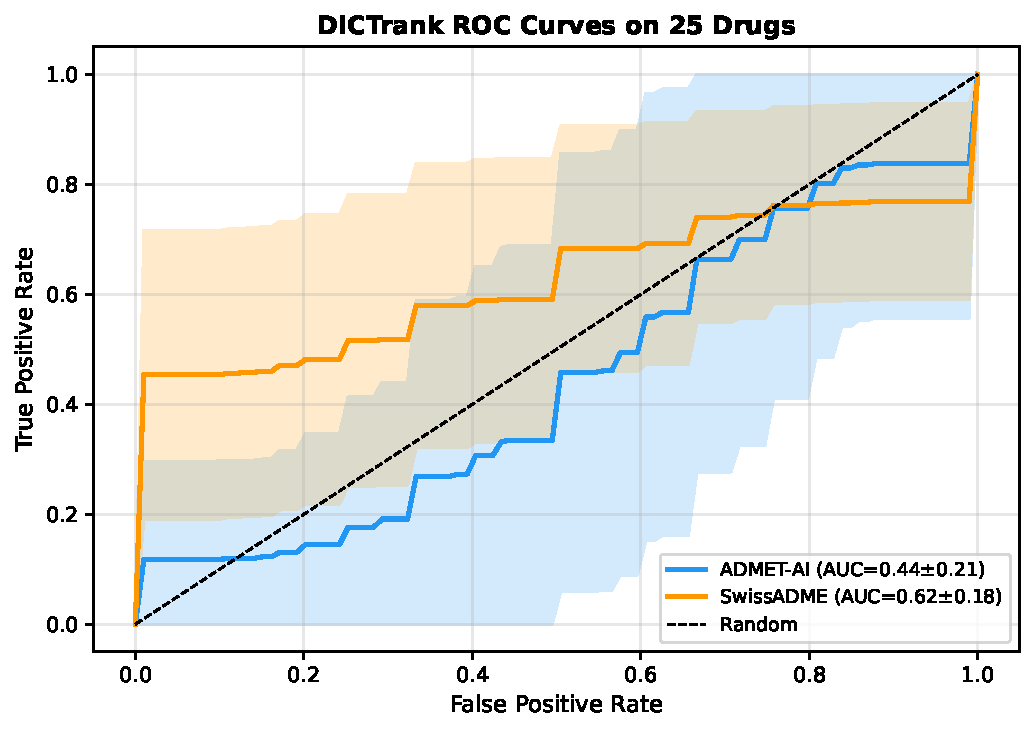
\includegraphics[width=\textwidth]{figures/dictrank_roc_25.pdf}
\end{minipage}
\caption{DICTrank accuracy and ROC (ADMET-AI: 25 drugs, SwissADME: 23 drugs).}
\end{figure}

\begin{figure}[H]
\centering
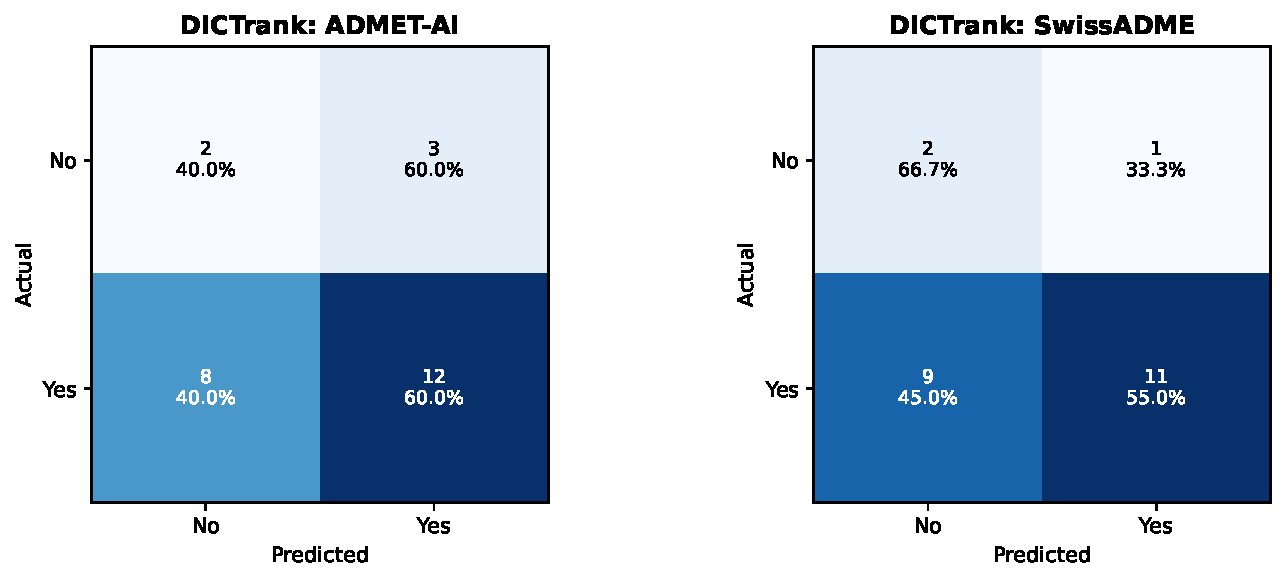
\includegraphics[width=0.85\textwidth]{figures/dictrank_confusion_matrices.pdf}
\caption{Confusion matrices for DICTrank models (ADMET-AI: 25 drugs, SwissADME: 23 drugs).}
\end{figure}

\begin{figure}[H]
\centering
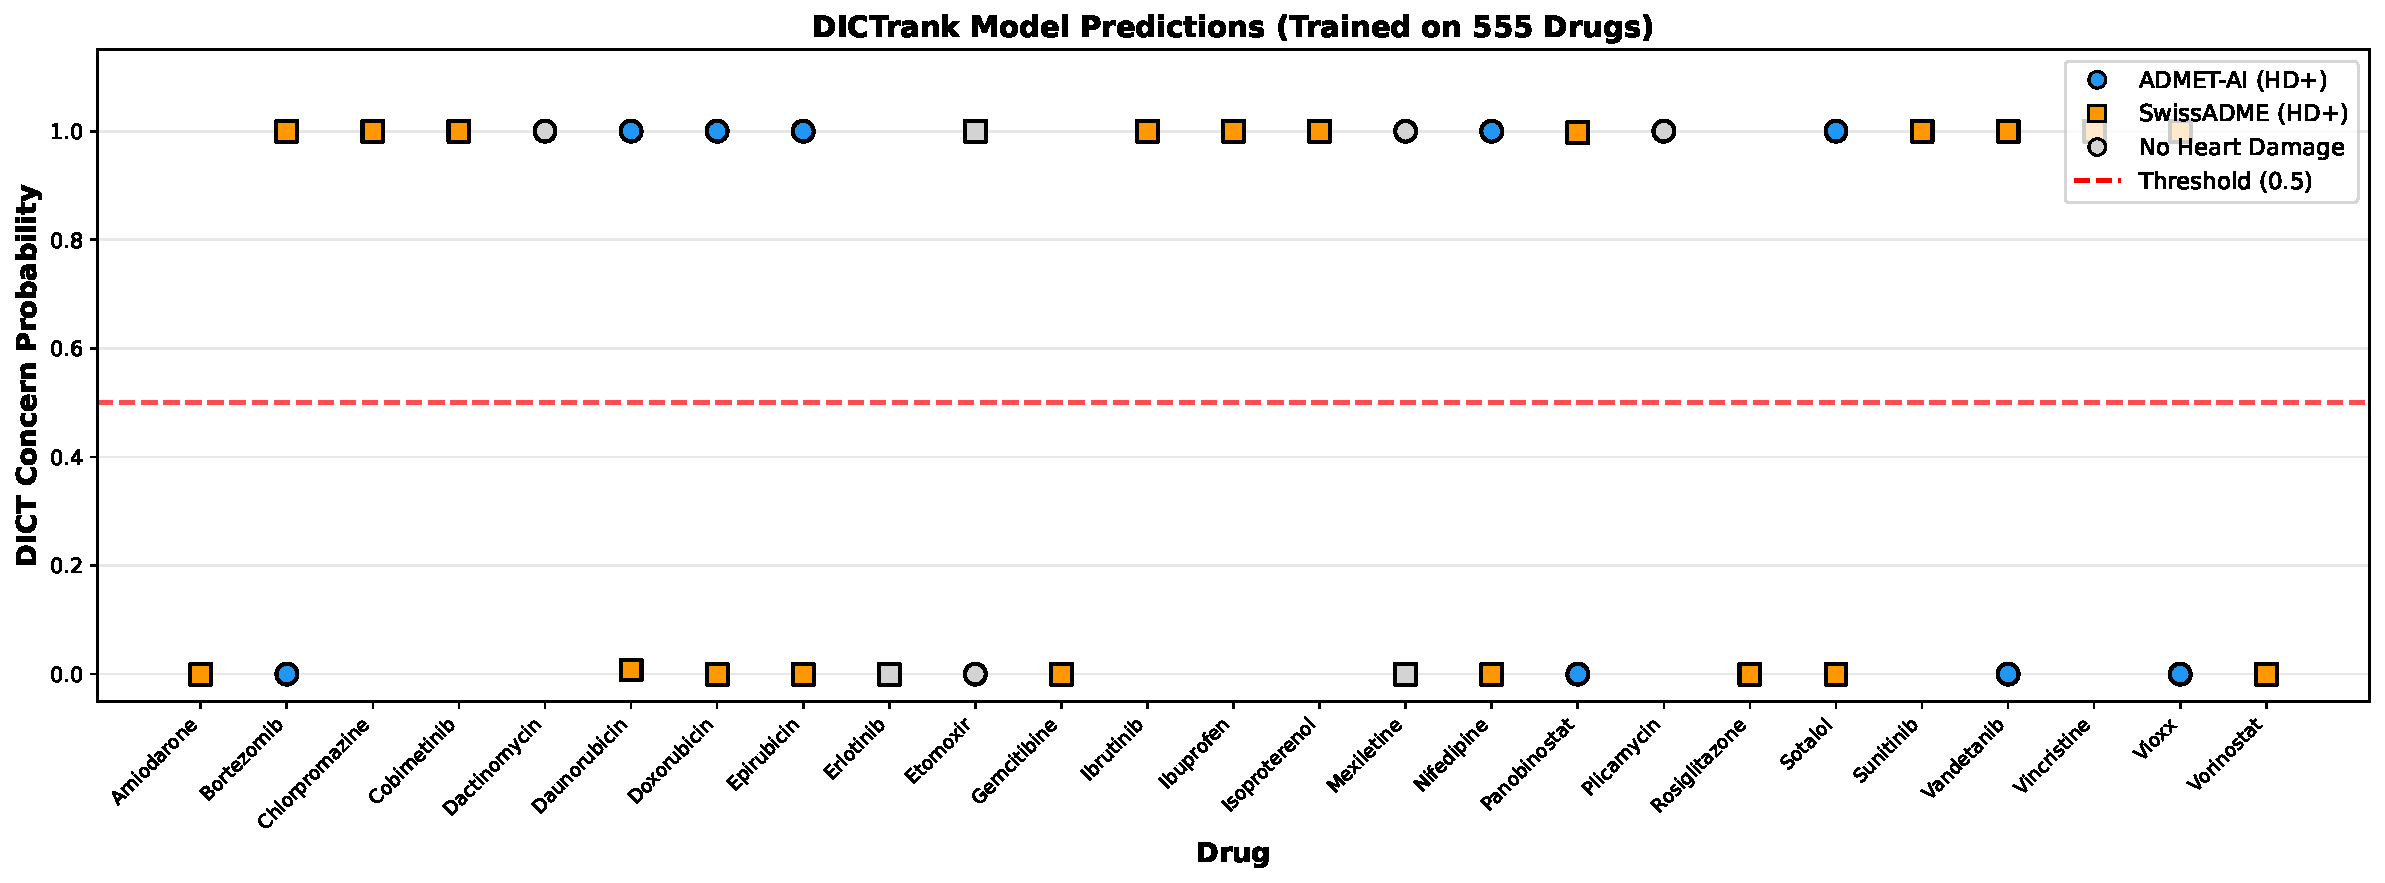
\includegraphics[width=\textwidth]{figures/dictrank_predictions.pdf}
\caption{DICTrank predictions for each drug. Circles = ADMET-AI, Squares = SwissADME*.}
\end{figure}
\textit{*SwissADME unavailable for Dactinomycin and Plicamycin due to size; SwissADME columns shown as ``--''.}

\begin{longtable}{lccccc}
\caption{Individual Drug Predictions (DICTrank Models)} \\
\toprule
\textbf{Drug} & \textbf{True HD} & \textbf{ADMET Prob} & \textbf{Pred} & \textbf{Swiss Prob} & \textbf{Pred} \\
\midrule
\endfirsthead
\toprule
\textbf{Drug} & \textbf{True HD} & \textbf{ADMET Prob} & \textbf{Pred} & \textbf{Swiss Prob} & \textbf{Pred} \\
\midrule
\endhead
    Amiodarone & Yes & 0.000 & Low & 0.000 & Low \\
    Bortezomib & Yes & 0.000 & Low & 1.000 & High \\
    Chlorpromazine & Yes & 1.000 & High & 1.000 & High \\
    Cobimetinib & Yes & 1.000 & High & 1.000 & High \\
    Dactinomycin & No & 1.000 & High & -- & -- \\
    Daunorubicin & Yes & 1.000 & High & 0.008 & Low \\
    Doxorubicin & Yes & 1.000 & High & 0.000 & Low \\
    Epirubicin & Yes & 1.000 & High & 0.000 & Low \\
    Erlotinib & No & 0.000 & Low & 0.000 & Low \\
    Etomoxir & No & 0.000 & Low & 1.000 & High \\
    Gemcitibine & Yes & 0.000 & Low & 0.000 & Low \\
    Ibrutinib & Yes & 1.000 & High & 1.000 & High \\
    Ibuprofen & Yes & 1.000 & High & 1.000 & High \\
    Isoproterenol & Yes & 1.000 & High & 1.000 & High \\
    Mexiletine & No & 1.000 & High & 0.000 & Low \\
    Nifedipine & Yes & 1.000 & High & 0.000 & Low \\
    Panobinostat & Yes & 0.000 & Low & 0.998 & High \\
    Plicamycin & No & 1.000 & High & -- & -- \\
    Rosiglitazone & Yes & 0.000 & Low & 0.000 & Low \\
    Sotalol & Yes & 1.000 & High & 0.000 & Low \\
    Sunitinib & Yes & 1.000 & High & 1.000 & High \\
    Vandetanib & Yes & 0.000 & Low & 1.000 & High \\
    Vincristine & Yes & 1.000 & High & 1.000 & High \\
    Vioxx & Yes & 0.000 & Low & 1.000 & High \\
    Vorinostat & Yes & 0.000 & Low & 0.000 & Low \\
\bottomrule
\end{longtable}

\section{LOOCV Models (25 Drugs)}

We retrain ADMET-AI and SwissADME models directly on the 25 Cardiac RODEO drugs.

\begin{table}[H]
\centering
\caption{LOOCV Model Performance}
\begin{tabular}{lcccccc}
\toprule
\textbf{Model} & \textbf{Accuracy} & \textbf{ROC AUC} & \textbf{TP} & \textbf{FN} & \textbf{TN} & \textbf{FP} \\
\midrule
ADMET-AI & 0.60 & 0.39 & 15 & 5 & 0 & 5 \\
SwissADME & 0.83 & 0.00 & 19 & 1 & 0 & 3 \\
\bottomrule
\end{tabular}
\end{table}

\begin{figure}[H]
\centering
\begin{minipage}{0.40\textwidth}
\centering
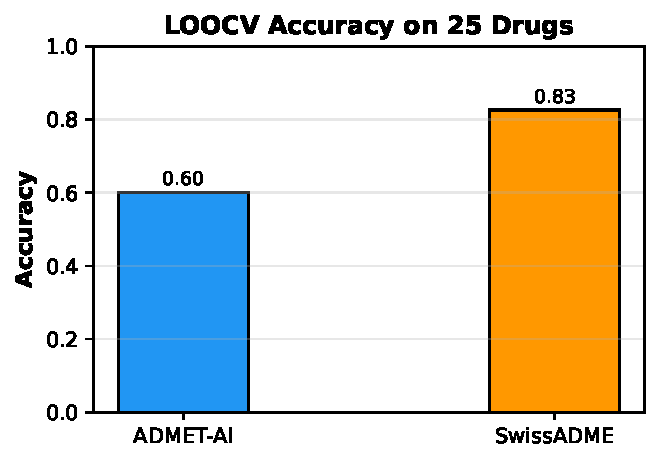
\includegraphics[width=\textwidth]{figures/loocv_accuracy_bar.pdf}
\end{minipage}
\hfill
\begin{minipage}{0.55\textwidth}
\centering
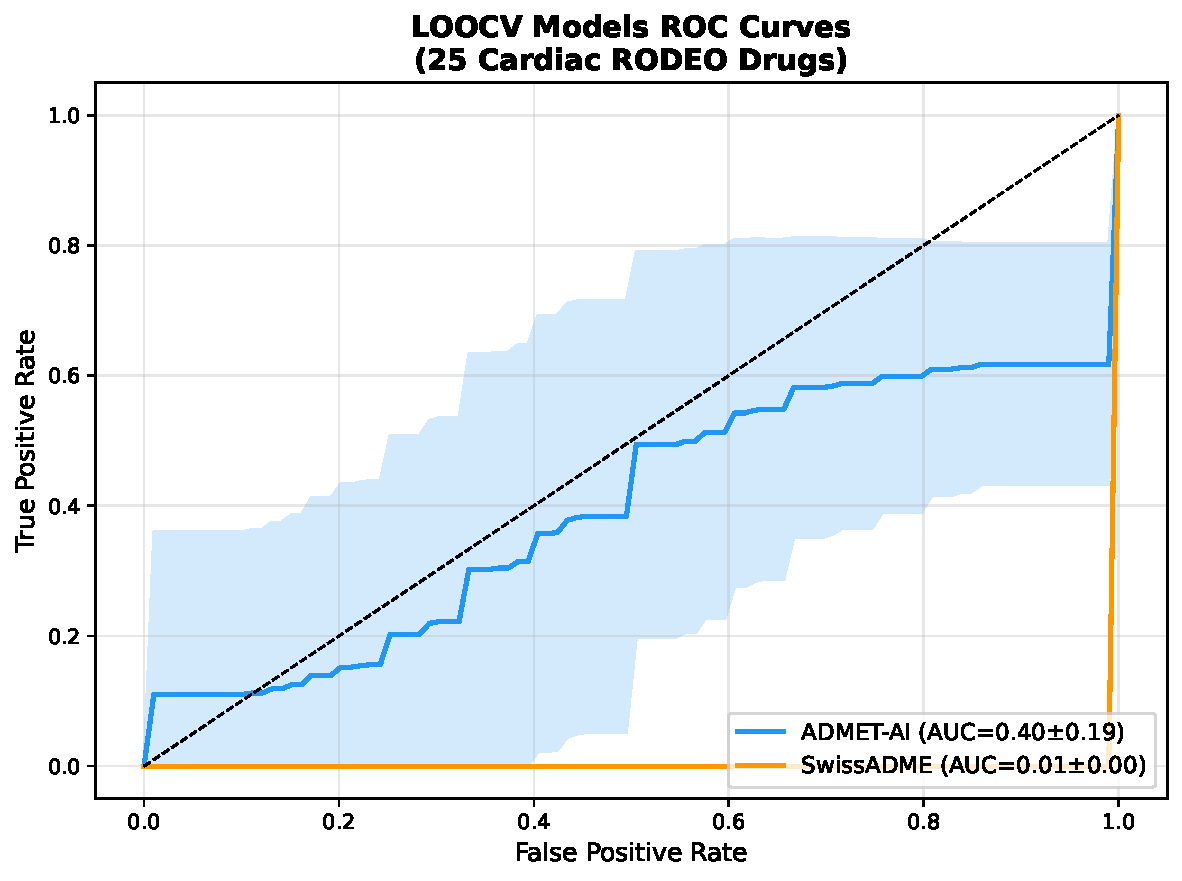
\includegraphics[width=\textwidth]{figures/loocv_roc.pdf}
\end{minipage}
\caption{LOOCV accuracy and ROC on 25 drugs.}
\end{figure}

\begin{figure}[H]
\centering
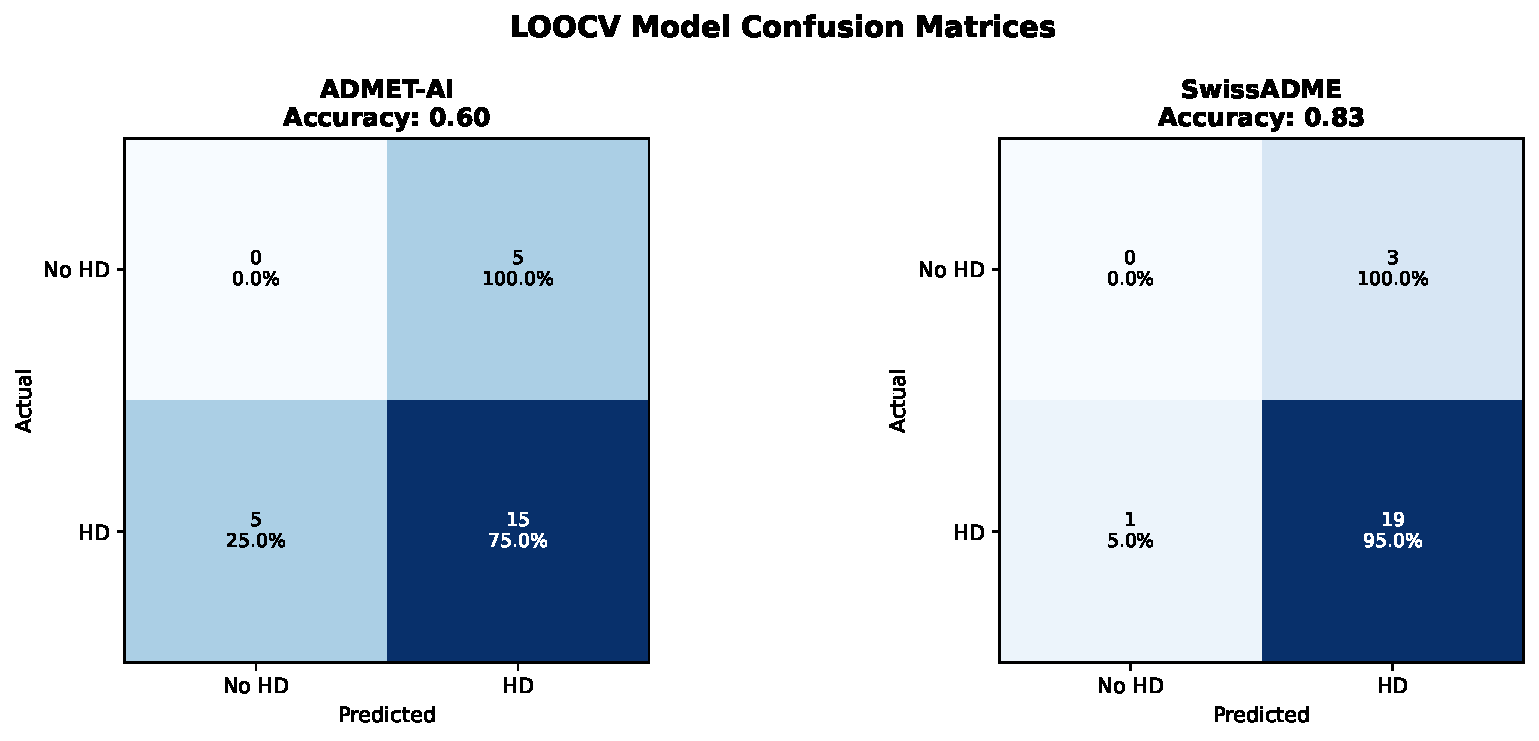
\includegraphics[width=\textwidth]{figures/loocv_confusion_matrices.pdf}
\caption{LOOCV confusion matrices (percent correct per class).}
\end{figure}
\textit{Note: Accuracy shown in the confusion-matrix titles is fold-averaged across LOOCV splits, while the matrix aggregates pooled predictions, so the diagonal may not match the title value.}

\begin{figure}[H]
\centering
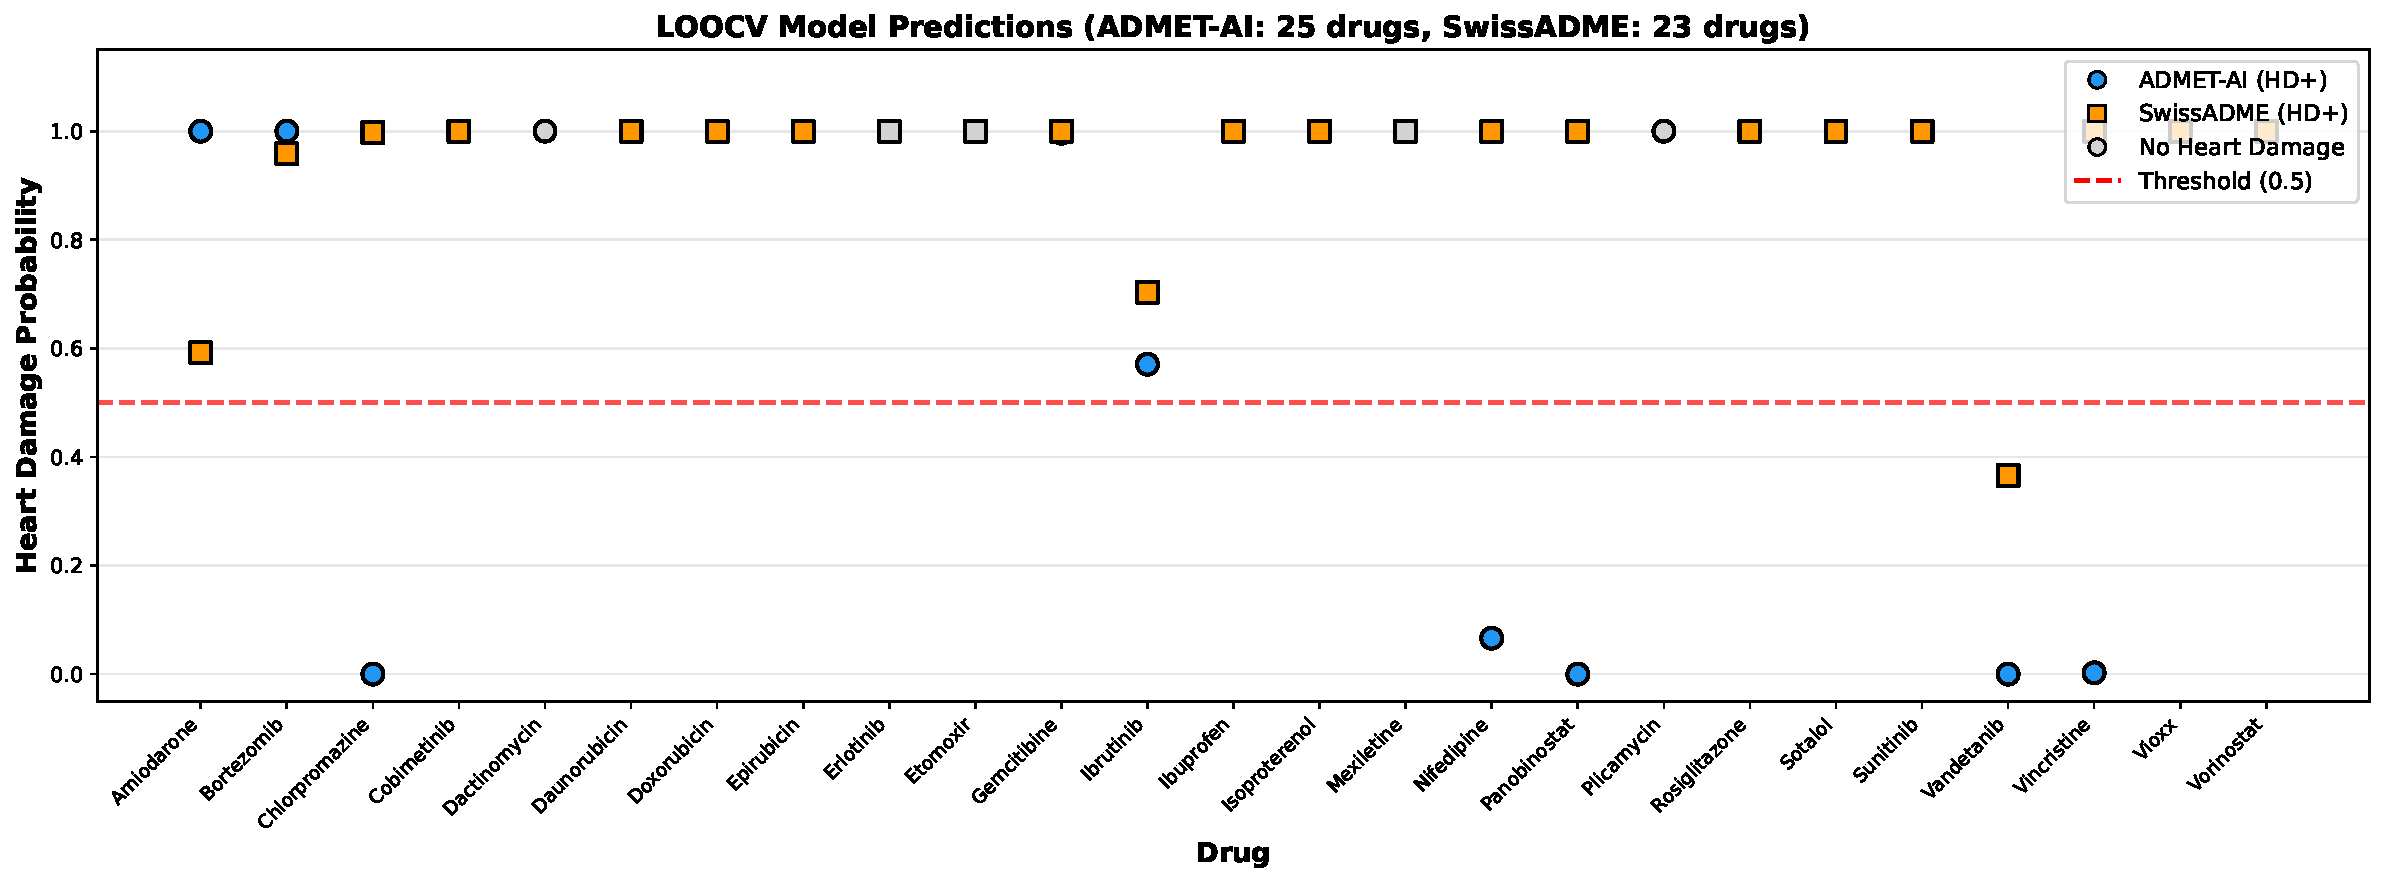
\includegraphics[width=\textwidth]{figures/loocv_predictions.pdf}
\caption{LOOCV predictions for each drug. Circles = ADMET-AI, Squares = SwissADME.}
\end{figure}


\section{Scaffold-Balanced CV Models (25 Drugs)}

\begin{table}[H]
\centering
\caption{Scaffold-Balanced CV Model Performance (25 Drugs)}
\begin{tabular}{lcccccc}
\toprule
\textbf{Model} & \textbf{Accuracy} & \textbf{ROC AUC (mean)} & \textbf{TP} & \textbf{FN} & \textbf{TN} & \textbf{FP} \\
\midrule
ADMET-AI & 0.54 & 0.44 & 27 & 11 & 0 & 12 \\
SwissADME & 0.80 & 0.38 & 40 & 20 & 15 & 20 \\
\bottomrule
\end{tabular}
\end{table}

\begin{figure}[H]
\centering
\begin{minipage}{0.40\textwidth}
\centering
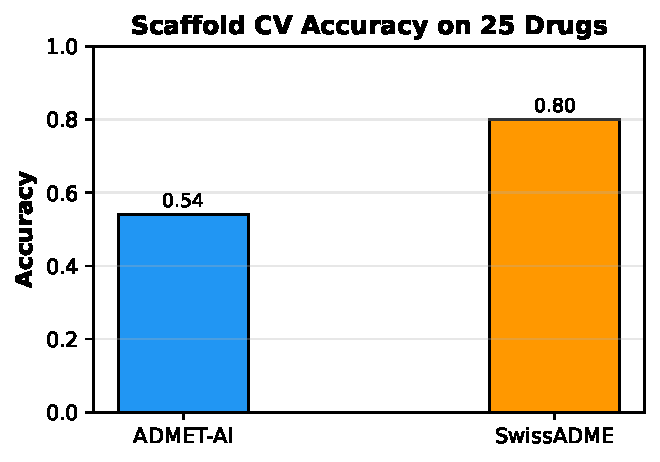
\includegraphics[width=\textwidth]{figures/scaffold_accuracy_bar.pdf}
\end{minipage}
\hfill
\begin{minipage}{0.55\textwidth}
\centering
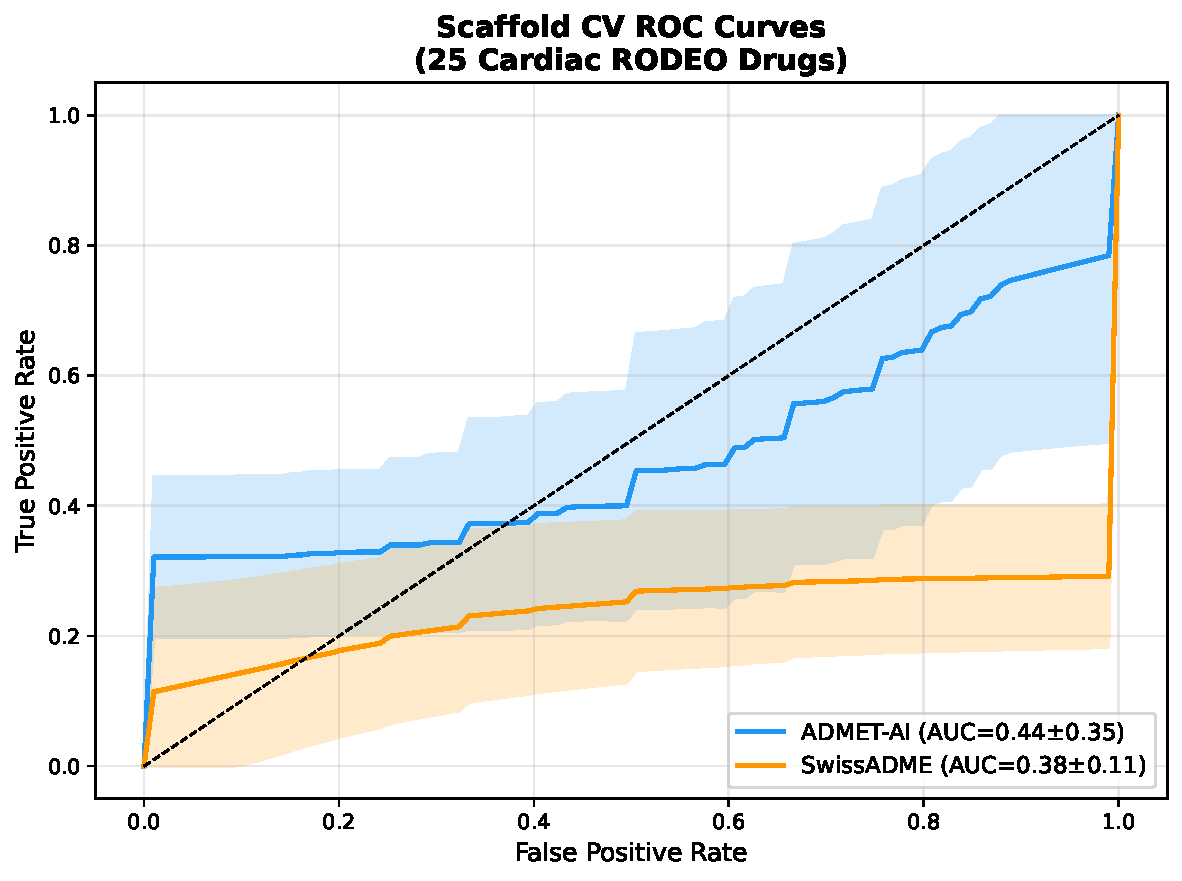
\includegraphics[width=\textwidth]{figures/scaffold_roc.pdf}
\end{minipage}
\caption{Scaffold CV accuracy and ROC on 25 drugs.}
\end{figure}

\begin{figure}[H]
\centering
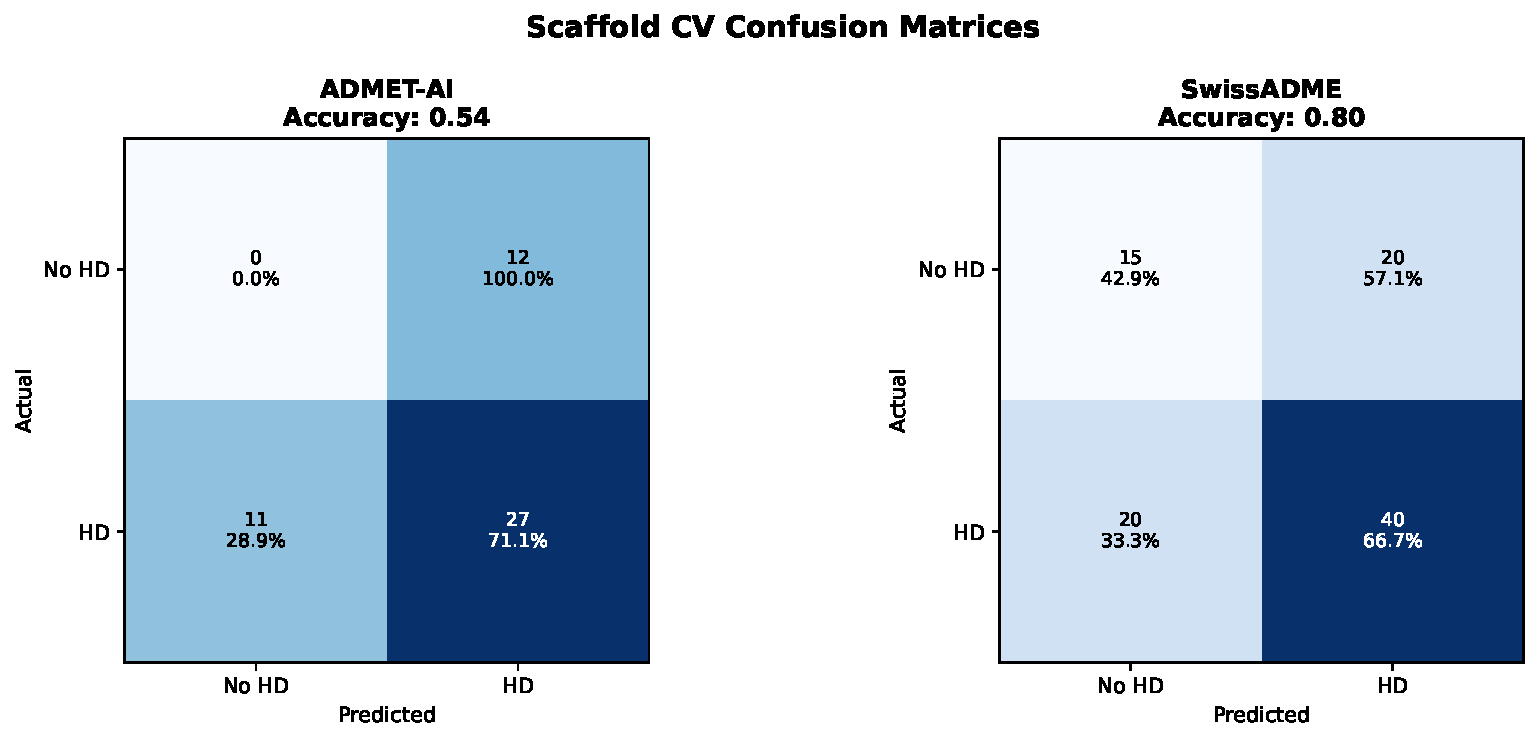
\includegraphics[width=\textwidth]{figures/scaffold_confusion_matrices.pdf}
\caption{Scaffold CV confusion matrices.}
\end{figure}
\textit{Note: Accuracy shown in the confusion-matrix titles is fold-averaged across scaffold splits, while the matrix aggregates counts across all scaffold splits (10 seeds), so the diagonal may not match the title value.}

\begin{figure}[H]
\centering
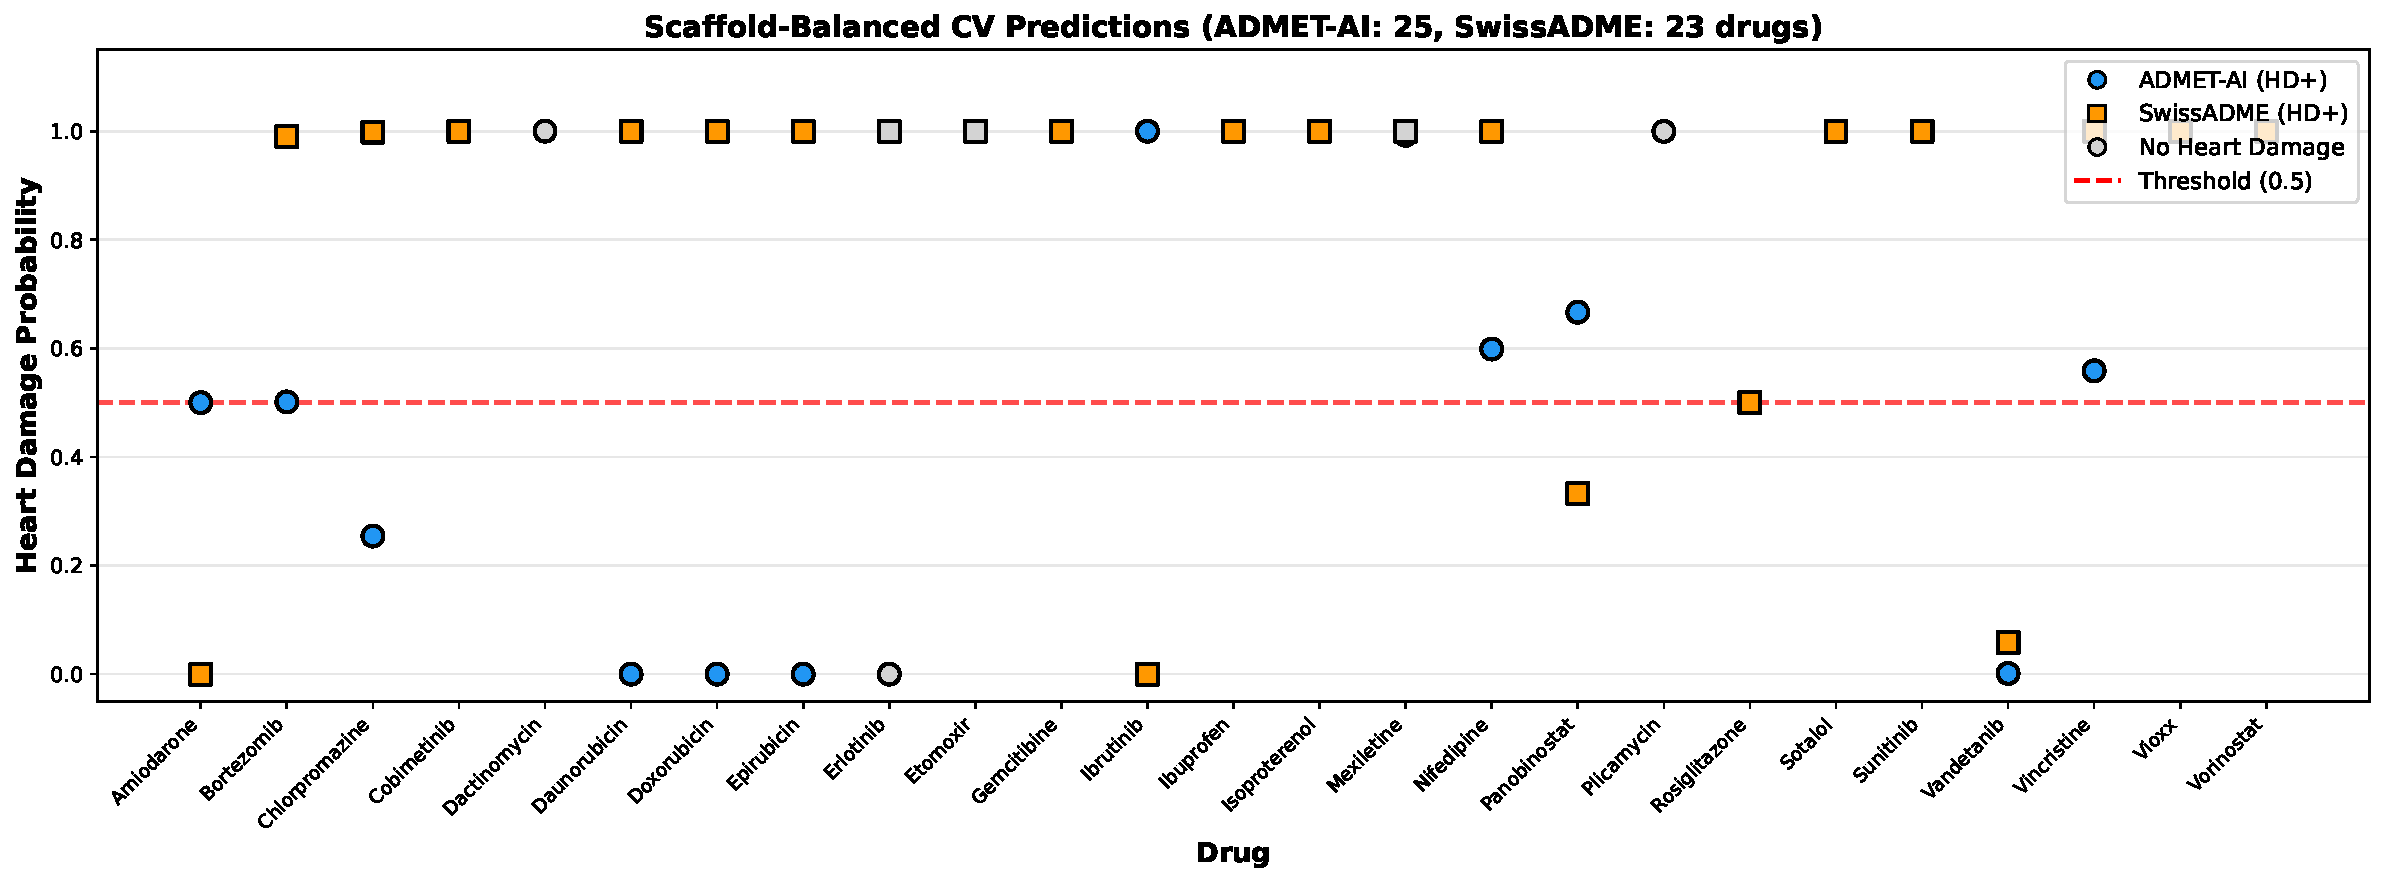
\includegraphics[width=\textwidth]{figures/scaffold_predictions.pdf}
\caption{Scaffold CV predictions for each drug. Circles = ADMET-AI, Squares = SwissADME.}
\end{figure}


\section{Organoid Model (LOOCV Comparison Pipeline)}

We include the organoid-trained model from the LOOCV model comparison pipeline for direct comparison on the 25 drugs.

\begin{table}[H]
\centering
\caption{Organoid Model Performance on 25 Drugs}
\begin{tabular}{lcc}
\toprule
\textbf{Model} & \textbf{Accuracy} & \textbf{ROC AUC} \\
\midrule
Organoid (GaussianNB) & 0.81 & 0.83 \\
\bottomrule
\end{tabular}
\end{table}

\begin{figure}[H]
\centering
\begin{minipage}{0.40\textwidth}
\centering
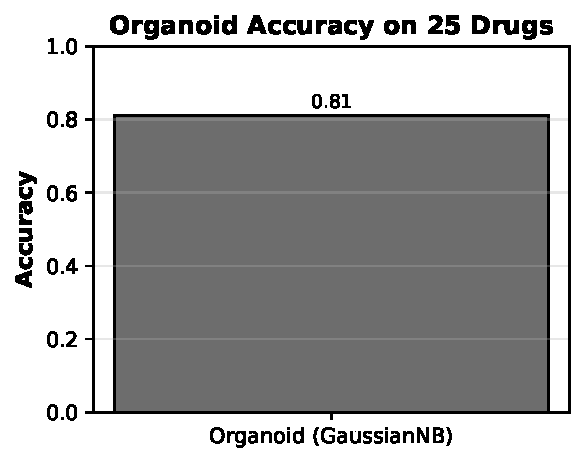
\includegraphics[width=\textwidth]{figures/organoid_accuracy_bar.pdf}
\end{minipage}
\hfill
\begin{minipage}{0.55\textwidth}
\centering
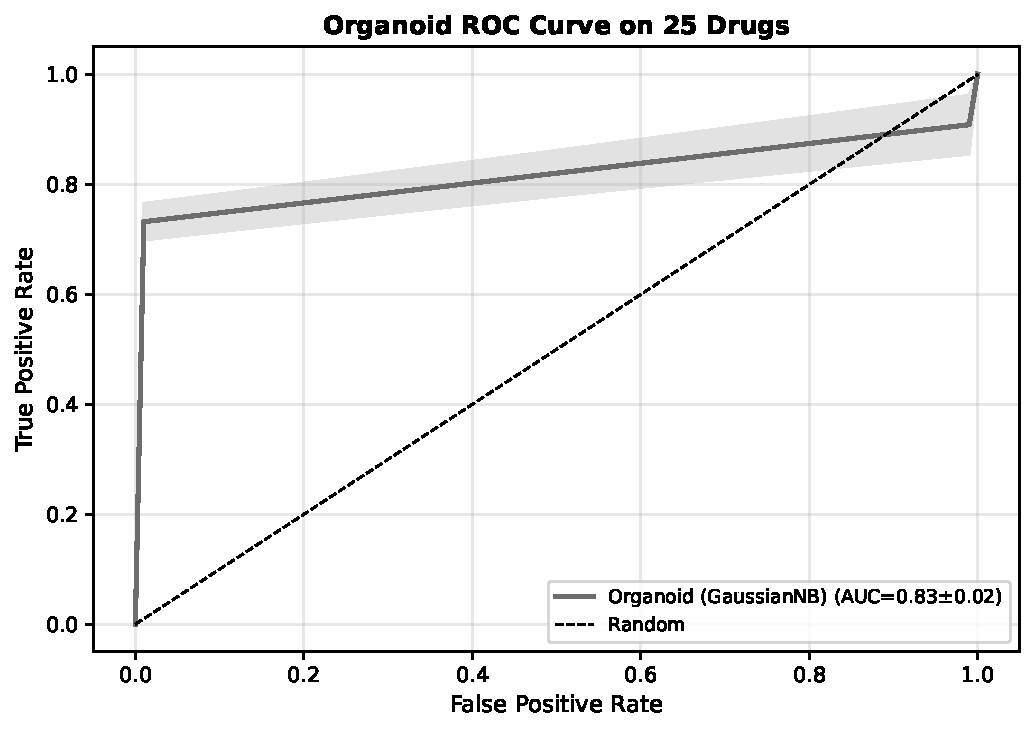
\includegraphics[width=\textwidth]{figures/organoid_roc.pdf}
\end{minipage}
\caption{Organoid accuracy and ROC on 25 drugs.}
\end{figure}


\begin{figure}[H]
\centering
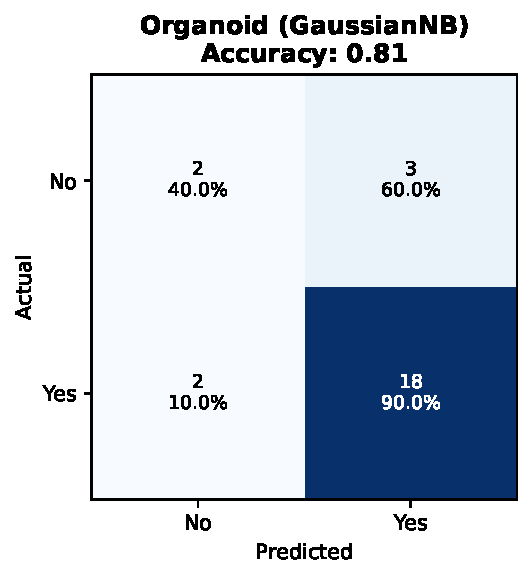
\includegraphics[width=0.6\textwidth]{figures/organoid_confusion_matrix.pdf}
\caption{Organoid confusion matrix (percent correct by class).}
\end{figure}


\section{Overall Comparison}

\begin{figure}[H]
\centering
\begin{minipage}{0.40\textwidth}
\centering
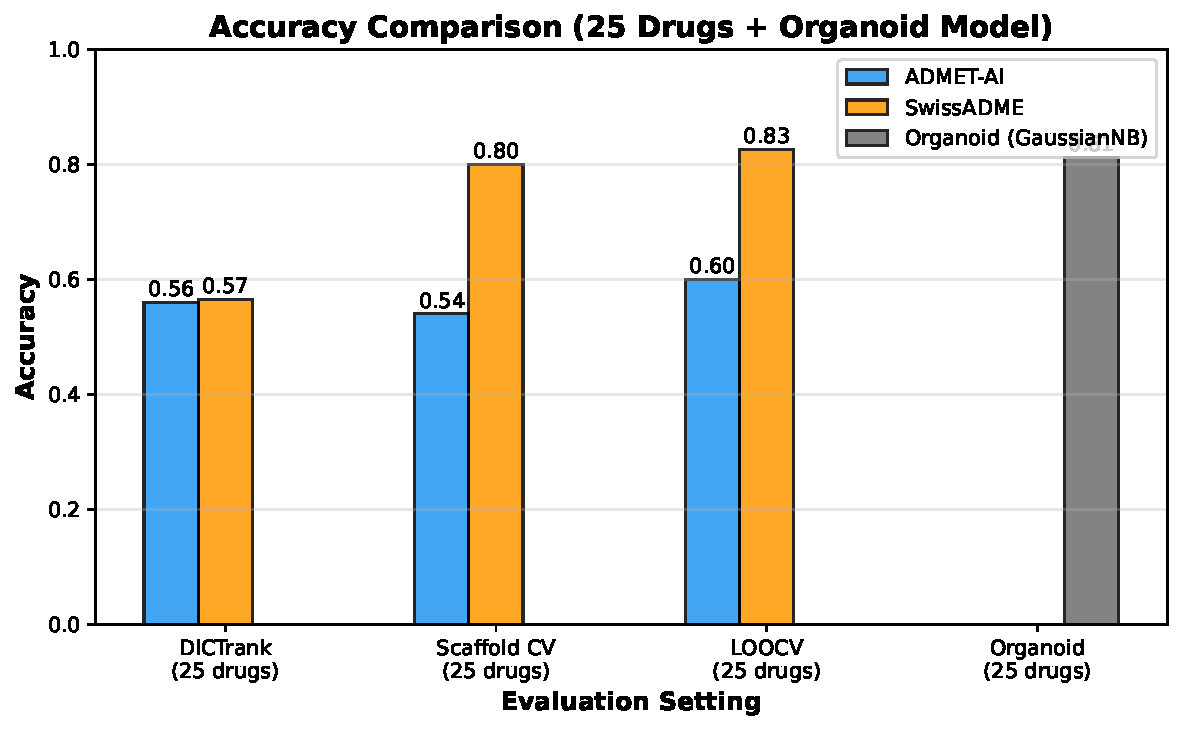
\includegraphics[width=\textwidth]{figures/accuracy_comparison.pdf}
\end{minipage}
\hfill
\begin{minipage}{0.55\textwidth}
\centering
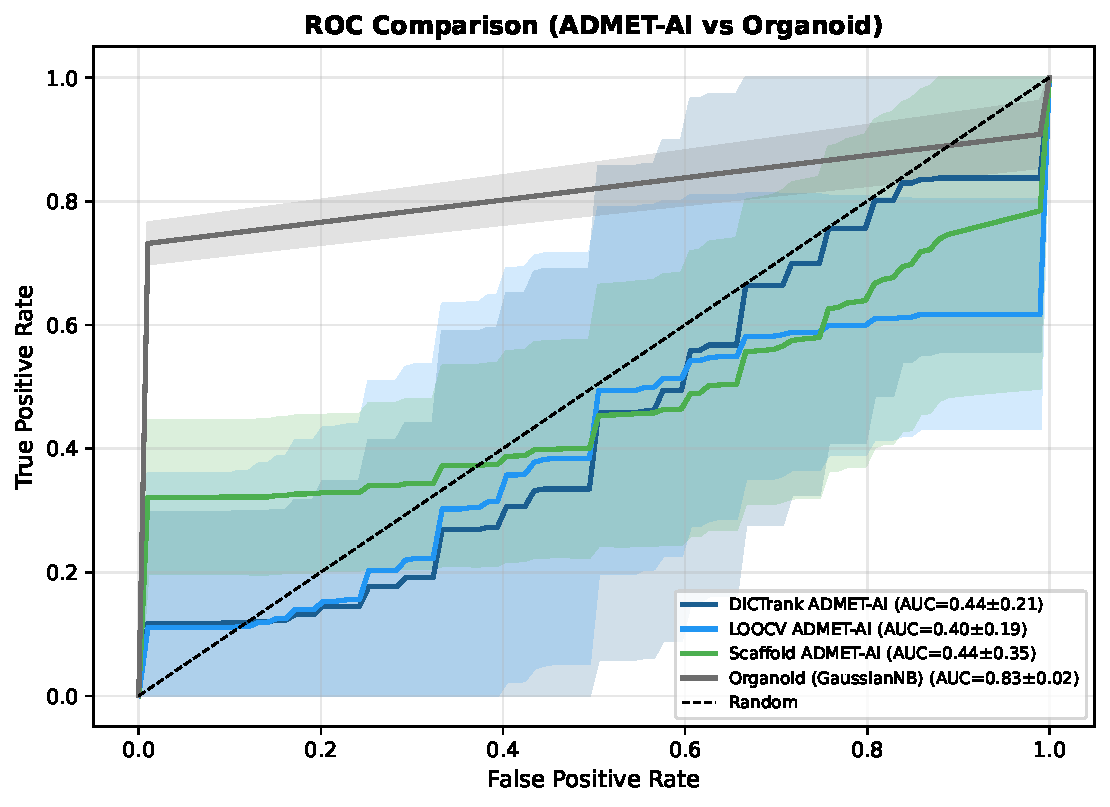
\includegraphics[width=\textwidth]{figures/overall_roc_comparison.pdf}
\end{minipage}
\caption{Overall comparison: accuracy and ROC (ADMET-AI vs organoid).}
\end{figure}

\begin{table}[H]
\centering
\caption{LOOCV vs DICTrank on 25 Drugs}
\begin{tabular}{lcccccc}
\toprule
\textbf{Model} & \textbf{DICTrank Acc} & \textbf{LOOCV Acc} & \textbf{$\Delta$ Acc} & \textbf{DICTrank AUC} & \textbf{LOOCV AUC} & \textbf{$\Delta$ AUC} \\
\midrule
ADMET-AI & 0.56 & 0.60 & +0.04 & 0.45 & 0.39 & -0.06 \\
SwissADME & 0.57 & 0.83 & +0.26 & 0.60 & 0.00 & -0.60 \\
\bottomrule
\end{tabular}
\end{table}

\begin{table}[H]
\centering
\caption{Scaffold CV vs DICTrank on 25 Drugs}
\begin{tabular}{lcccccc}
\toprule
\textbf{Model} & \textbf{DICTrank Acc} & \textbf{Scaffold Acc} & \textbf{$\Delta$ Acc} & \textbf{DICTrank AUC} & \textbf{Scaffold AUC} & \textbf{$\Delta$ AUC} \\
\midrule
ADMET-AI & 0.56 & 0.54 & -0.02 & 0.45 & 0.44 & -0.01 \\
SwissADME & 0.57 & 0.80 & +0.23 & 0.60 & 0.38 & -0.23 \\
\bottomrule
\end{tabular}
\end{table}


\section{Comprehensive Performance Metrics with Standard Deviations}

The following table summarizes all methods with their CV-based standard deviations.
Standard deviations represent variability across cross-validation folds, providing
a measure of model performance stability.

\begin{table}[H]
\centering
\caption{Comprehensive Performance Metrics (Mean $\pm$ Std)}
\small
\begin{tabular}{llcccc}
\toprule
\textbf{Method} & \textbf{Model} & \textbf{Accuracy} & \textbf{ROC AUC} & \textbf{F1} & \textbf{MCC} \\
\midrule
DICTrank & ADMET-AI & 0.56 & 0.45 & -- & -- \\
DICTrank & SwissADME & 0.57 & 0.60 & -- & -- \\
\midrule
Scaffold & ADMET-AI & 0.54 $\pm$ 0.24 & 0.44 $\pm$ 0.35 & 0.66 $\pm$ 0.26 & -0.21 $\pm$ 0.32 \\
Scaffold & SwissADME & 0.80 $\pm$ 0.18 & 0.38 $\pm$ 0.11 & 0.88 $\pm$ 0.12 & 0.00 $\pm$ 0.00 \\
\midrule
LOOCV & ADMET-AI & 0.60 & 0.39 $\pm$ 0.19 & -- & -- \\
LOOCV & SwissADME & 0.83 & 0.00 $\pm$ 0.00 & -- & -- \\
\midrule
Organoid & Organoid (GaussianNB) & 0.81 $\pm$ 0.03 & 0.83 $\pm$ 0.02 & 0.89 $\pm$ 0.02 & 0.36 $\pm$ 0.08 \\
\bottomrule
\end{tabular}
\end{table}

\textit{Note: DICTrank and LOOCV methods do not report F1/MCC std. Organoid std values from 5-fold CV on 25 drugs.
Scaffold CV std values computed from 10-fold scaffold-balanced cross-validation.}

\section{Feature Importance (SHAP, ADMET-AI)}

\clearpage
\subsection{DICTrank}
\begin{figure}[H]
\centering
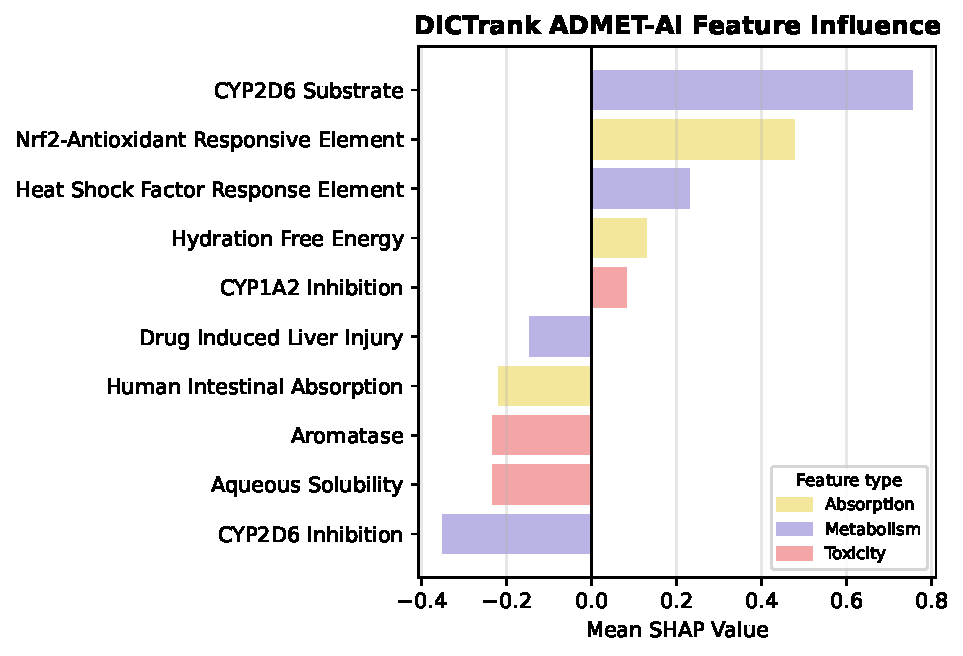
\includegraphics[width=0.85\textwidth]{figures/dictrank_shap_features.pdf}
\caption{DICTrank ADMET-AI feature influence (paper-aligned ordering).}
\end{figure}

\clearpage
\subsection{LOOCV}
\begin{figure}[H]
\centering
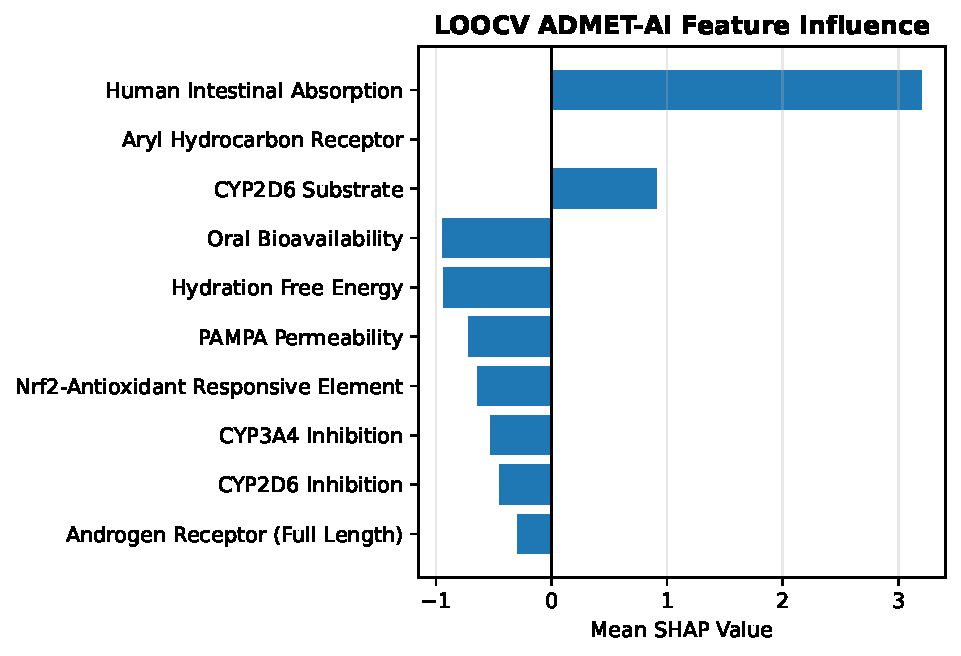
\includegraphics[width=0.85\textwidth]{figures/loocv_shap_features.pdf}
\caption{LOOCV ADMET-AI feature influence.}
\end{figure}

\clearpage
\subsection{Scaffold CV}
\begin{figure}[H]
\centering
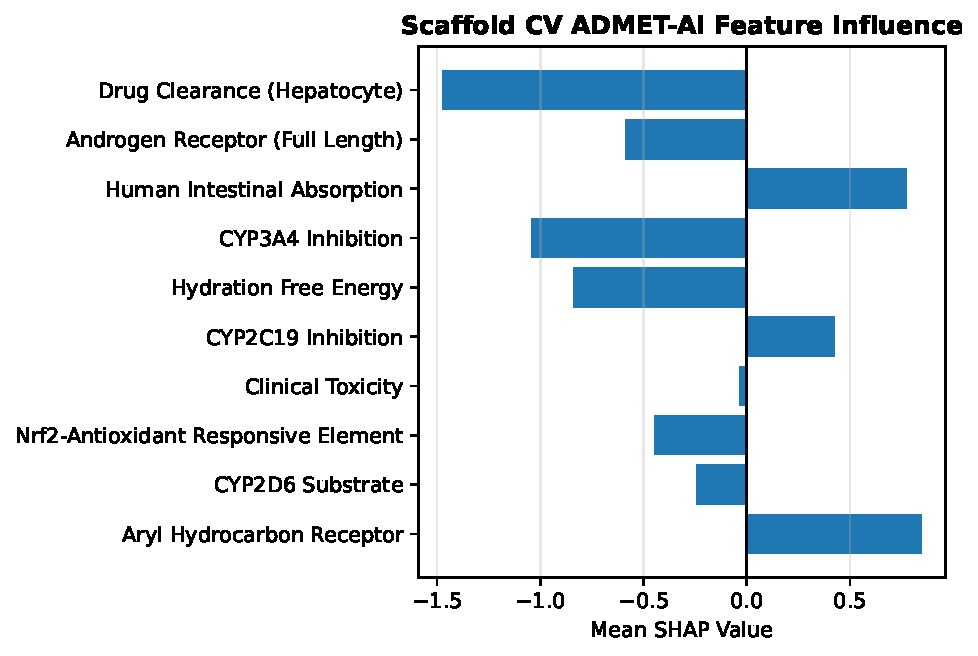
\includegraphics[width=0.85\textwidth]{figures/scaffold_shap_features.pdf}
\caption{Scaffold CV ADMET-AI feature influence.}
\end{figure}


\section*{Supplementary: Scripts Used}
\begin{itemize}
    \item \texttt{ADMET\_Comparison/Scripts/retrain\_dictrank\_models.py} --- Retrains DICTrank models with scaffold-balanced CV and saves training metrics.
    \item \texttt{ADMET\_Comparison/Scripts/predict\_retrained\_dictrank.py} --- Runs trained DICTrank models on the 25-drug feature tables.
    \item \texttt{ADMET\_Comparison/Scripts/run\_predictions\_v2.py} --- Generates ADMET-AI features for Cardiac RODEO SMILES and DICT predictions.
    \item \texttt{ADMET\_Comparison/Scripts/predict\_swissadme.py} --- Trains SwissADME model and predicts DICT concern for 25 drugs.
    \item \texttt{ADMET\_Comparison/Scripts/full\_analysis.py} --- Assembles plots, tables, and the LaTeX report.
    \item \texttt{Prediction\_Models/loocv\_model\_comparison.py} --- LOOCV pipeline and ROC Excel export used for organoid comparisons.
\end{itemize}


\section*{References}
Mukherjee P, et al. (2025). ADMET-AI Enables Interpretable Predictions of Drug-Induced Cardiotoxicity. \textit{Clinical Pharmacology \& Therapeutics}.

\end{document}
